% Dokumentinformationen
\title{ElMasch - Zusammenfassung}
\author{Gregor Dengler}
\documentclass[10pt,twoside,a4paper,fleqn]{article}

% Header
\include{header/zusammenfassung}


% Document
\begin{document}
\setcounter{tocdepth}{2} 	%Es wird nur bis Subsection im Inhaltsverzeinichs angezeigt
\tableofcontents 				%Inhaltsverzeichnis
\newpage
\section{Die elektrodynamischen Grundgesetze}
\subsection{Elektrische Kraft und elektrisches Feld}

\begin{minipage}{0.4 \linewidth}
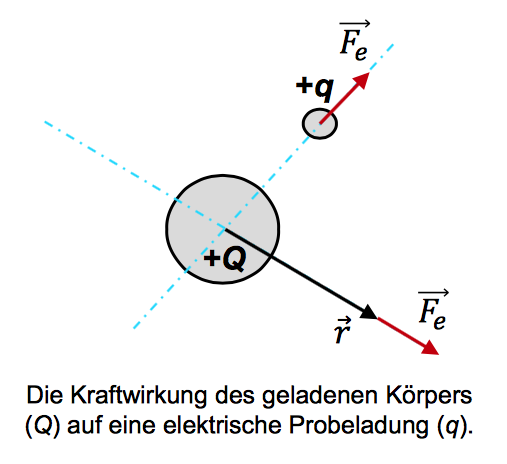
\includegraphics[width = \linewidth]{./Pics/VL1/elKraft}
\end{minipage}
\begin{minipage}{0.5 \linewidth}
Die elektrische Kraft zwischen unendlichen parallelen Leitern:

$\vec{F_{e}} = \frac{1}{2 \pi \epsilon} \cdot \frac{Qq}{r} \cdot \vec{r_{0}} (\frac{N}{m})$ \\

$\epsilon$ - dielektrische Permittivität \\
$\epsilon_{0}$ - die Permittivität des Vakuums \\
$\epsilon_{0} = 8.85 \cdot 10^{-12}$ $(\frac{As}{Vm})$ \\
$Q,q$ - Linienladungsdichten $(\frac{C}{m})$ \\
$\vec{r_{0}} = \frac{\vec{r}}{|\vec{r}|} $ - Einheitsvektor\\
\end{minipage}

\begin{minipage}{0.5 \linewidth}
Das elektrische Feld wird als die elektrische Kraft auf die Einheitsladung definiert:
\begin{equation}
\vec{E} = \frac{\vec{F_{e}}}{q} \ (\frac{V}{m})
\vec{E} = \frac{1}{2 \pi \epsilon} \cdot \frac{Q}{r} \cdot \vec{r_{0}}(\frac{V}{m})
\end{equation}
\end{minipage}
\begin{minipage}{0.4 \linewidth}
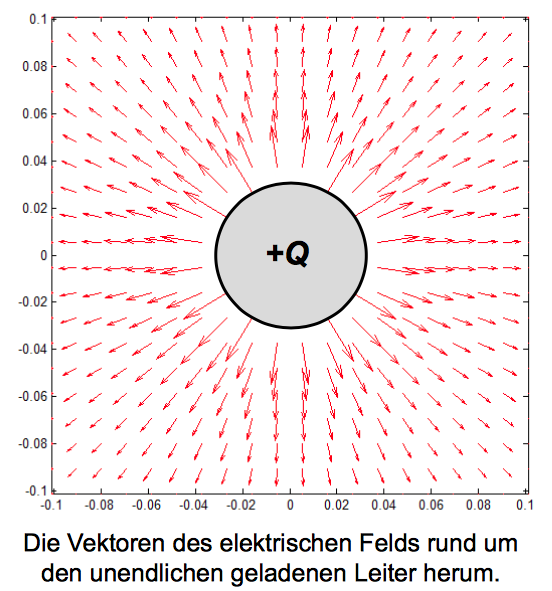
\includegraphics[width = \linewidth]{./Pics/VL1/elFeld}
\end{minipage}

\subsection{Elektrisches Potential und elektrische Spannung}

\begin{minipage}{0.5 \linewidth}
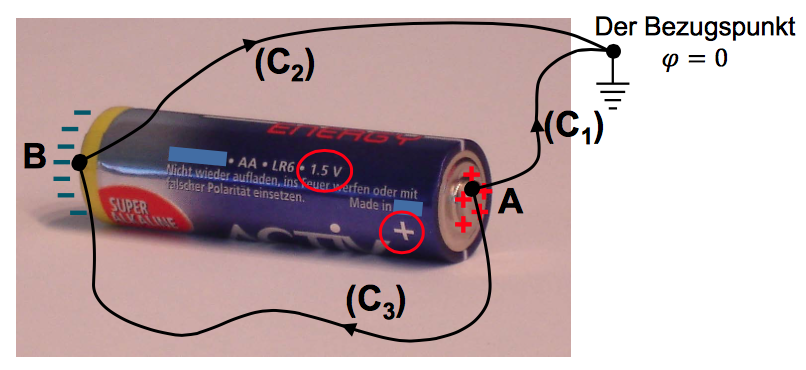
\includegraphics[width = \linewidth]{./Pics/VL1/elPot}
\end{minipage}
\begin{minipage}{0.5 \linewidth}
Die elektrische Potentiale:\\ $\varphi$ = $\int_{A}^{Bezugspunkt} \vec{E} \cdot \vec{dl}$, $\varphi_{B} = \int_{B}^{Bezugspunkt} \vec{E} \cdot \vec{dl}$
Die elektrische Spannung:
$U_{AB} = \int_{A}^{B} \vec{E} \cdot \vec{dl} = \varphi_{A} - \varphi_{B}$  (V)

Das elektrische Potential eines Ortes ist eigentlich die Arbeit, die für die Bewegung der Einheitsladung vom Bezugspunkt zum Ort nötig ist.
 \end{minipage}

\subsection{Elektrische Strom}

\begin{minipage}{0.4 \linewidth}
Elektrische Strom:

$I = \frac{dQ}{dt}$ (A)

Elektrischer Widerstand:

$R = \frac{U}{I}$  ($\Omega$)
\end{minipage}
\begin{minipage}{0.6 \linewidth}
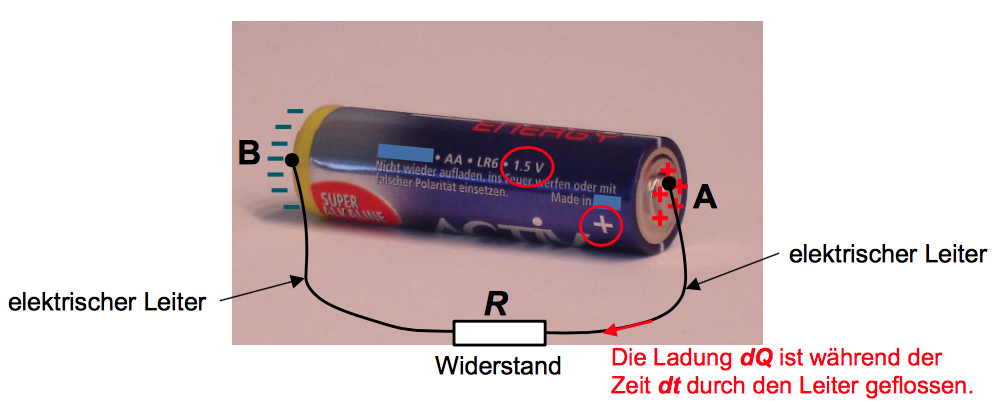
\includegraphics[width = \linewidth]{./Pics/VL1/elStrom}
 \end{minipage}
 
 \subsection{Magnetische Kraft}
 
 \begin{minipage}{0.5 \linewidth}
 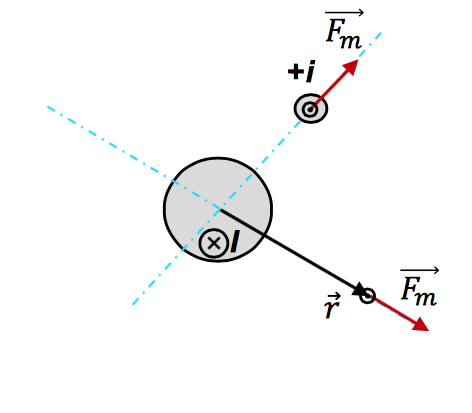
\includegraphics[width = \linewidth]{./Pics/VL1/elMag}
 \end{minipage}
 \begin{minipage}{0.5 \linewidth}
Die magnetische Kraft zwischen unendlich parallelen Leitern:
$ \vec{F_{m}} = \frac{\mu}{2 \pi} \cdot \frac{Ii}{r} \cdot \vec{r_{0}}$  ($\frac{N}{m}$) \\
$\mu$ - magnetische Permeabilität \\
$\mu_{0}$ - die Permeabilität des Vakuums \\
$\mu_{0} = 4 \pi \cdot 10^{-7}$ ($\frac{N}{A^{2}}$) \\
$I,i$ - elektrische Ströme (A) \\
$\vec{r_{0}} = \frac{\vec{r}}{|\vec{r}|} $ - Einheitsvektor \\
  \end{minipage}
  
  \begin{minipage}{0.5 \linewidth}
	Das magnetische Feld ist klein Potenzialfeld, sondern ein quellenfreies Feld: \\
	$\vec{F_{m}} = \mu \cdot i \cdot \vec{l_{0}} \times \vec{H}$  ($\frac{N}{m}$) \\
	$\vec{H} = \frac{I}{2 \pi} \cdot \frac{\vec{L_{0}} \times \vec{r_{0}}}{r}$  $(\frac{A}{m})$\\
	$\vec{r_{0}} = \frac{\vec{r}}{|\vec{r}|} $ - Einheitsvektor \\
	$\vec{L_{0}}, \vec{l_{0}}$ - Einheitsvektoren der Stromleiter \\
   \end{minipage}
   \begin{minipage}{0.5 \linewidth}
   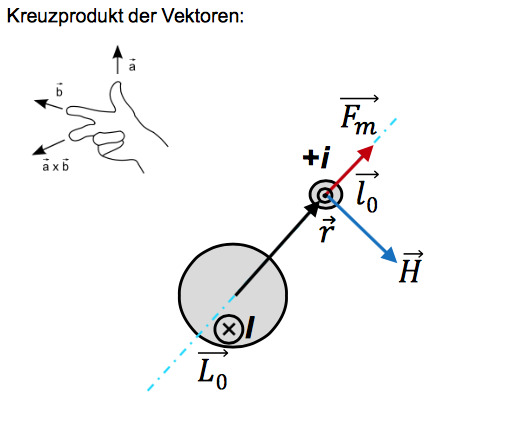
\includegraphics[width = \linewidth]{./Pics/VL1/magFeld}
    \end{minipage}
    
    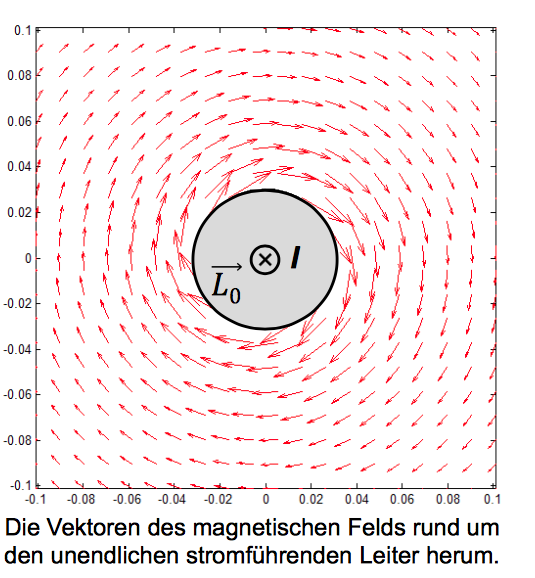
\includegraphics[width = 0.3\linewidth]{./Pics/VL1/magFeld2}
    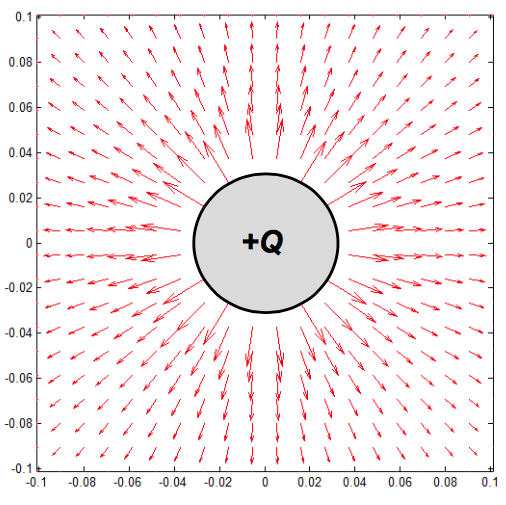
\includegraphics[width = 0.3\linewidth]{./Pics/VL1/magFeld3}
    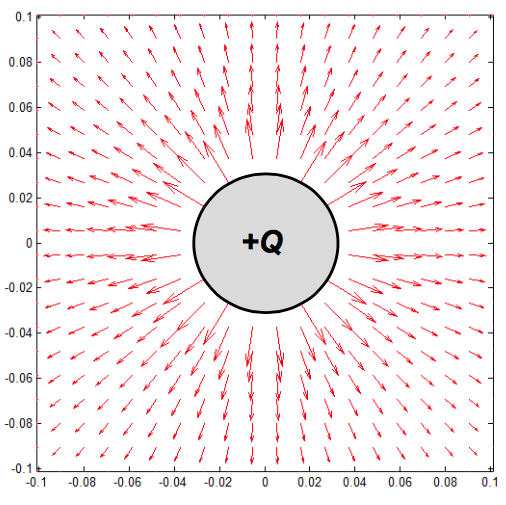
\includegraphics[width = 0.3\linewidth]{./Pics/VL1/magFeld3}
    
    $\vec{E} = \frac{1}{2 \pi \epsilon} \cdot \frac{Q}{r} \cdot \vec{r_{0}}$  ($\frac{V}{m}$) \\
    $\vec{H} = \frac{I}{2 \pi} \cdot \frac{\vec{L_{0}} \times \vec{r_{0}}}{r}$  $(\frac{A}{m})$\\
    	
\subsection{Elektrische und magnetische Kraft im Vergleich}
    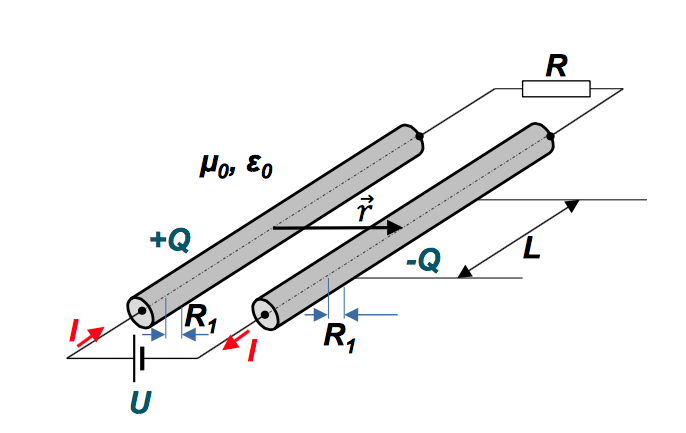
\includegraphics[width = 0.35\linewidth]{./Pics/VL1/elMagVergleich}
    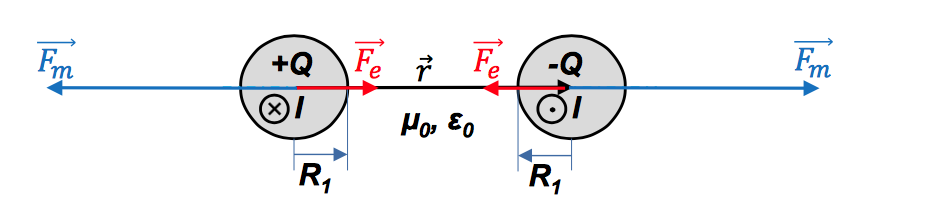
\includegraphics[width = 0.6\linewidth]{./Pics/VL1/elMagVergleich2}
    
\subsubsection{Berechnungsbeispiel}
\begin{tabular}{ll}
Die wichtige Annahme: & $r >> R_1$ \\
Die geometrischen Daten: & $R_{1}$ = 10mm, r = 100mm, L = 1000mm\\
Die elektrischen Daten:& U = 1V, I = 1A  \\
Die Kräfte pro Längeneinheit: &$F_{e} = \frac{\pi \cdot \epsilon_{0} \cdot U^{2}}{2 \cdot r \cdot (ln\frac{r-R_{1}}{R_{1}})^{2}} = 2.88 \cdot 10^{11}$ $(\frac{N}{m})$ \\
&$F_{m} = \frac{\mu_{0} \cdot I^{2}}{2 \cdot \pi \cdot r} = 2.00 \cdot 10^-6$ $(\frac{N}{m})$ \\
\end{tabular}

Die wichtigsten Schlussfolgerungen:
\begin{enumerate}
\item Der Absolutbetrag der magnetischen Kraft pro Längen- und Stromeinheit ist ungefähr $7 \cdot 10^{4}$ mal grösser als der entsprechende Betrag der elektrischen Kraft pro Längen- und Spannungseinheit.
\item Um die Kraft von 1 ($\frac{N}{m}$) in dieser Anordnung zu erzeugen ist entweder der Strom von ungefähr 700A oder die Spannung von ungefähr 600'000 V notwendig. 
\item \textbf{Die Argumente 1 und 2 deuten darauf hin, dass die magnetische Kraft für die Energieumwandlung besser als die elektrische Kraft geeignet ist.} Deswegen basieren die modernen elektrischen Maschinen hauptsächlich auf der magnetischen Kraft.
\end{enumerate}
    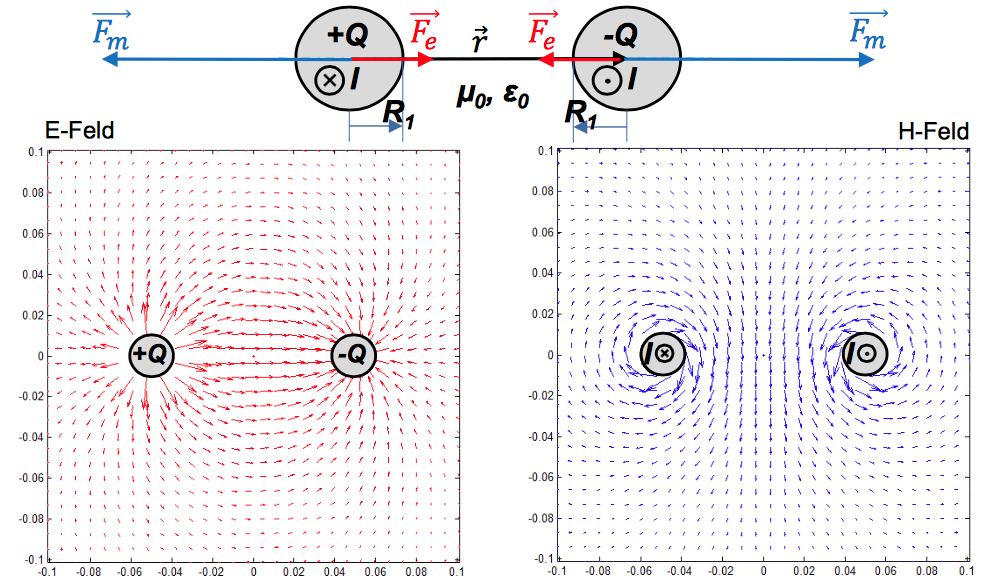
\includegraphics[width = 0.75\linewidth]{./Pics/VL1/magKraft}
    
\subsection{Begriffe und Kennwerte des Magnetfelds}
\begin{minipage}{0.2 \linewidth}
    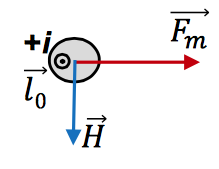
\includegraphics[width =\linewidth]{./Pics/VL1/magKraft2}
\end{minipage}
\begin{minipage}{0.8 \linewidth}
Die Kraft auf den stromführenden Leitern im Magnetfeld:\\

$\vec{F_m} = \mu \cdot i \cdot \vec{l_0} /times \vec{H}$  $(\frac{N}{m})$ = $ i \cdot \vec{l_0} \times \vec{B}$  ($\frac{N}{m}$) \\

Die magnetische Kraft ist nicht nur vom H-Feld abhängig, sondern die magnetische Eigenschaft des Materials spielen dabei auch eine wichtige Rolle. Deswegen wird \textbf{die magnetische Induktion} und \textbf{die magnetische Flussdichte} definiert:\\

$ \vec{B} = \mu \cdot \vec{H} = \mu_0 \cdot \mu_r \cdot \vec{H}$  ($T = \frac{Vs}{m^2}$) \\

$\mu_0 = 4 \pi \cdot 10^{-7}$  ($\frac{Vs}{Am} = \frac{Tm}{A}$) \\

$\mu_r = \frac{\mu}{\mu_0}$ - die relative Permeabilität des Materials \\
\end{minipage}

\begin{minipage}{0.2 \linewidth}
    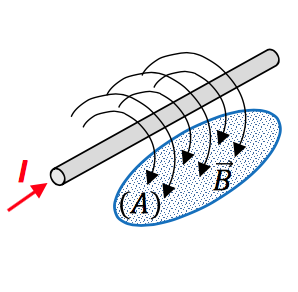
\includegraphics[width =\linewidth]{./Pics/VL1/magFluss}
\end{minipage}
\begin{minipage}{0.8 \linewidth}
\textbf{Der magnetische Fluss} ist als der Fluss des Vektors $\vec{B}$ durch eine Fläche A definiert:\\

$\Phi = \int\int_{(A)} \vec{B} \cdot \vec{dA}$ \\

Wenn der Fluss $ \Phi$ durch eine Spuhle mit $N$ Windungen fliesst, wird der gesamte Fluss der Spule denn als \textbf{der verkettete magnetische Fluss} gennant: \\

$\Psi = N \cdot \Phi$ \\

Der zeitvariierende magnetische Fluss durch eine Spule mit $N$ Windungen \textbf{induziert die folgende elektrische Spannung} in der Spule.\\

$U_{ind} = - \frac{d \Psi}{dt} = -N \frac{d \Phi}{dt}$ (V)
\end{minipage}

\begin{minipage}{0.2 \linewidth}
    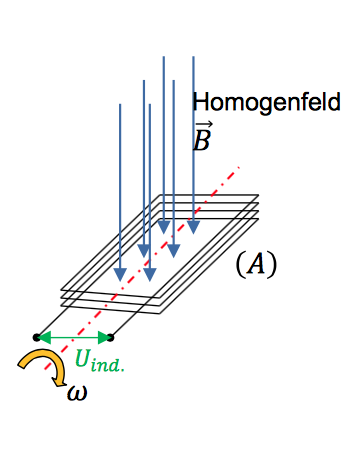
\includegraphics[width =\linewidth]{./Pics/VL1/elGen}
\end{minipage}
\begin{minipage}{0.8 \linewidth}
\textbf{Das Wirkungsprinzip eines elektromagnetischen Generators} ist hier dargestellt. Der Generator besteht im Wesentlichen aus einer Spule mit $N$ Windungen, die sich im magnetischen Homogenfeld um ihre Achse mit der konstanten Winkelgeschwindigkeit $\omega$ dreht:\\

$\Psi (t) = N \cdot \int\int_{(A)} \vec{B} \cdot \vec{dA} = N \cdot B \cdot A \cdot cos(\omega t) $ \\

\textbf{Die induzierte Spannung} der Spule kann wie folgt gerechnet werden: \\

$U_{ind.} = - \frac{d\Psi}{dt} = \omega \cdot N \cdot B \cdot A \cdot sin(\omega t)$  $(V)$
\end{minipage}

\subsection{Zusammenfassung}

\begin{itemize}
\item Die elektrische Kraft wirkt auf eine elektrische Ladung im elektrsichen Fremdfeld.
\item Die magnetische Kraft wirkt auf einen stromführenden Leiter im magnetischen Fremdfeld.
\item Die magnetische Kraft zwischen zwei parallelen stromdurchflossenen Leitern pro Strom- und Längeneinheit ist viel höher als die entsprechende elektrische Kraft zwischen den Leitern pro Spannung- und Längeneinheit.
\item Der elektrische Wechselstrom erzeugt das magnetische Wechselfeld.
\item In einer Spule, die sich im magnetischen Wechselfeld befindet, wird die elektrische Wechselspannung induziert.
\end{itemize}
\section{Magnetkreis-Begriff, Permanentmagnet, Reluktanzkraft}
\subsection{Magnetische Durchflutung}
\begin{minipage}{0.2 \linewidth}
    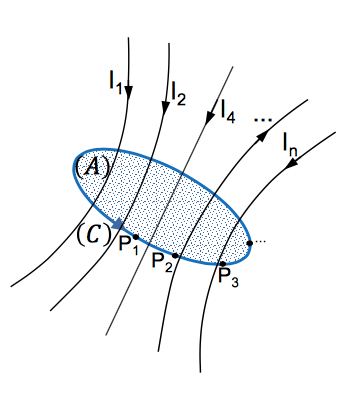
\includegraphics[width =\linewidth]{./Pics/VL2/magDurchflutung}
\end{minipage}
\begin{minipage}{0.8 \linewidth}
\textbf{Die magnetische Durchflutung} einer von der Kontur (C) umrandetetn Fläche (A) ist der gesamte Strom, der durch diese Fläche fliesst: \\

$\Theta = \sum_{k = 1}^{n} I_k$\\

Nach dem \textbf{Durchflutungsgesetz} muss das Linienintegral des magnetischen Felds entlang der Kontur (C) die entsprechende elektrische Durchlutung ergeben: \\

$\oint \vec{H} \cdot \vec{dl} = \sum_{k=1}^{n} I_k = \Theta$\\

Diese Gleichung ist eine sehr wichtige Verknüpfung zwischen dem Magnetfeld und dem elektrischen Strom. Sie wird sehr oft \textbf{für die Berechnung des Magnetfelds} einer angegebenen Erreger-Anordnung eingesetzt. 
\end{minipage}
\subsection{Magnetische Spannung}
\begin{minipage}{0.2 \linewidth}
    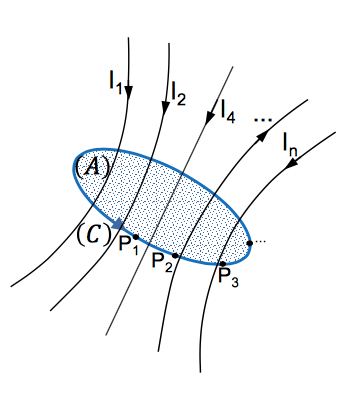
\includegraphics[width =\linewidth]{./Pics/VL2/magDurchflutung}
\end{minipage}
\begin{minipage}{0.8 \linewidth}
Um das Linienintegral einfacher zu rechnen sollte die Integrationskurve (C) passen definiert und aufgeteilt werden: \\

$\oint_{(C)} \vec{H} cdot \vec{dl} = \oint_{P_1}^{P_2} \vec{H} \cdot \vec{dl} + \oint_{P_2}^{P_3} \vec{H} \cdot \vec{dl}  + \cdots +\oint_{P_{m-1}}^{P_m} \vec{H} \cdot \vec{dl} $ \\

Der Definition der elektrischen Spannung zufolge, wird die magnetische Spannung wie folgt definiert: \\

$V_m = \int^B_A \vec{H} \cdot \vec{dl}$ \\

Die Aufteilung der Integrationskurve(C) wird normalerweise so durchgeführt, dass eine Summation anstatt der Integration ergeben wird: \\

$\oint_{(C)} \vec{H} \cdot \vec{dl} = H_1 \cdot l_1 + H_2 \cdot l_2 + H_3 \cdot l_3 + \cdots = V_{m1} + V_{m2} + V_{m3} + \cdots$
\end{minipage}

\subsection{Magnetischer Widerstand}
\begin{minipage}{0.2 \linewidth}
    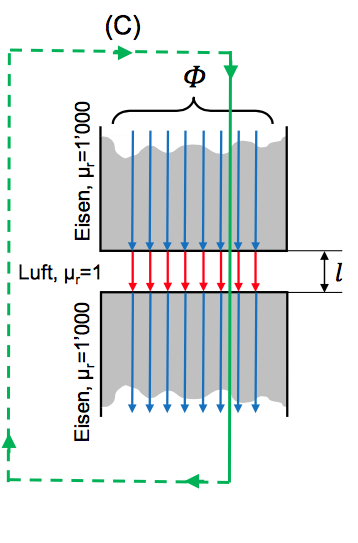
\includegraphics[width =\linewidth]{./Pics/VL2/magR}
\end{minipage}
\begin{minipage}{0.8 \linewidth}
Der magnetische Fluss durch einen Luftspalt zwischen den Eisenblöcken lässt sich wie folgt angeben:\\

$\Phi_{1Eisen} = \Phi_{Luft} = \Phi_{2Eisen} \Rightarrow B_{1Eisen} =  B_{Luft} = B_{2Eisen}$ \\

Jedoch ist die magnetische Permeabilität von Eisen etwa 1000 mal grösser als die Permeabilität von Luft, was in dieser Anordnung das magnetische Feld im Luftspalt bestimmt: \\

$B_{1Eisen} = B_{Luft} \Rightarrow \mu_{0} \cdot \mu_{rEisen} \cdot H_{Eisen} = \mu_0 \cdot \mu_{rLuft} \cdot H_{Luft}$ \\

$H_{Luft} = \frac{\mu_{rEisen}}{\mu_{rLuft}} \cdot H_{Eisen} \Rightarrow H_{Luft} \approx 1'000 \cdot H_{Eisen}$ \\

Offenbar ist das magnetische Feld in der Luft viel grösser als das entsprechende Feld im Eisen. Das bedeutet, dass die magnetische Spannung entlang einer Flusslinie mit den Luftstrecken der Linie bestimmt wird: \\

$\oint_{(C)} \vec{H} \cdot \vec{dl} = H_{Eisen} \cdot l_{Eisen} + H_{Luft} \cdot l_{Luft} \approx H_{Luft} \cdot l_{Luft} = V_{mLuft}$ \\

Die magnetische Spannung des Luftspalts spielt eine wichtige Rolle in jeder Anordnung mit einem Eisenkern: \\

$\oint_{(C)} \vec{H} \cdot \vec{dl} \approx H_{Luft} \cdot l_{Luft} = V_{mLuft}$ \\

Der Definition des elektrischen Widerstands zufolge, wird den magnetischen Widerstand wie folgt definiert: \\

$R_m = \frac{V_m}{\Phi}$ \\

Wenn $A$ die auf den magnetischen Fluss senkrechte Fläche des Luftspaltes ist, lässt sich denn der magnetische Widerstand des Luftspaltes wie folgt angeben: \\

$R_m = \frac{H_0 \cdot l}{B_0 \cdot A} = \frac{H_0 \cdot l}{\mu_0 \cdot H_0 \cdot A} = \frac{l}{\mu_0 \cdot A}$
 \end{minipage}

\subsection{Magnetkreis}

Die Annahme der Feldberechnung: \\
Das magnetische Feld in der Spule ist \textbf{viel grösser} als draussen und das Feld in der Spule \textbf{ist homogen}. Die Annahmen sind dann realistisch, wenn $L >> R$ ist.\\

$\oint_{(C)} \vec{H} \cdot \vec{dl} \approx H \cdot L = N \cdot I \Rightarrow H = \frac{N \cdot I}{L}, B = \mu_0 \cdot \frac{N \cdot I}{L}$

\begin{minipage}{0.5 \linewidth}
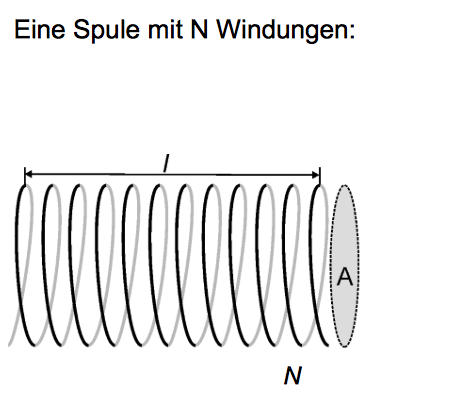
\includegraphics[width = \linewidth]{./Pics/VL2/spule}
\end{minipage}
\begin{minipage}{0.5 \linewidth}
Das magnetische Feld und die magnetische Flussdichte der Spule: \\

$H = \frac{N \cdot I}{L}$ \\

Für die Spule mit den folgenden geometrischen Daten: \\

R = 0.1m, L = 0.27m, N = 10, I = 1A \\

wird das folgende magnetische Feld gerechnet: \\

$H = 37.4 \frac{A}{m}, B = 46.5 \mu T $\\

$\mu_0 = 4 \pi \cdot 10^{-1}$ ($\frac{Tm}{A}$)
\end{minipage}

\subsubsection{H-Feld im Luftspalt (vereinfachte Herleitung)}
\begin{minipage}{0.4 \linewidth}
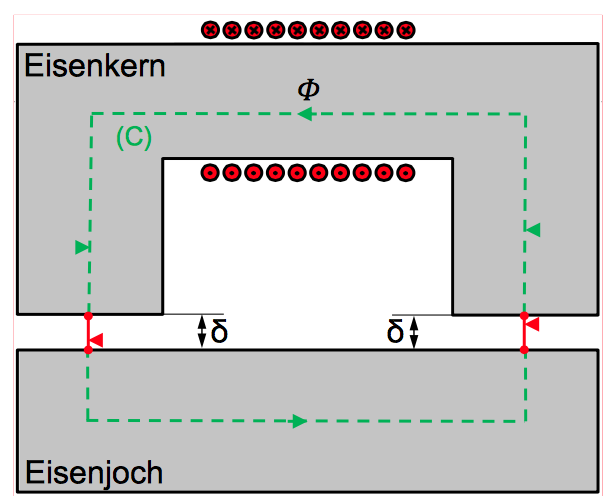
\includegraphics[width = \linewidth]{./Pics/VL2/magKreis}
\end{minipage}
\begin{minipage}{0.6 \linewidth}
Gemäss dem Durchflutungsgesetz lässt sich das Magnetfeld eines Magnetkreises wie folgt angeben: \\

$\oint_{(C)} \vec{H} \cdot \vec{dl} = H_{Fe} \cdot l_{Fe} + 2 \cdot \delta \cdot H_{\delta}  = I \cdot N $ \\

Wie schon präsentiert, ist in dieser Anordnung das magnetische Feld im Luftspalt viel grösser als das entsprechende Feld im Eisen: \\

$H_{\delta} \approx \cdot H_{Fe} \Rightarrow H_{\delta} = \frac{I \cdot N}{2 \delta} $ \\

$B_{\delta} = \mu_0 \frac{I \cdot N}{2 \delta} $ \\

Ein Magnetkreis mit einer stromdurchflossenen Spule erzeugt einen magnetischen Fluss, der den entsprechenden Magnetfluss ohne Magnetkreis mehrere Grössenordnungen überschiesst. 
\end{minipage}

\subsubsection{Beispiele}
\includegraphics[width = 0.8 \linewidth]{./Pics/VL2/magKreisBeispiele}

\subsubsection{H-Feld im Luftspalt (Allgemeine Herleitung)}
\begin{minipage}{0.4 \linewidth}
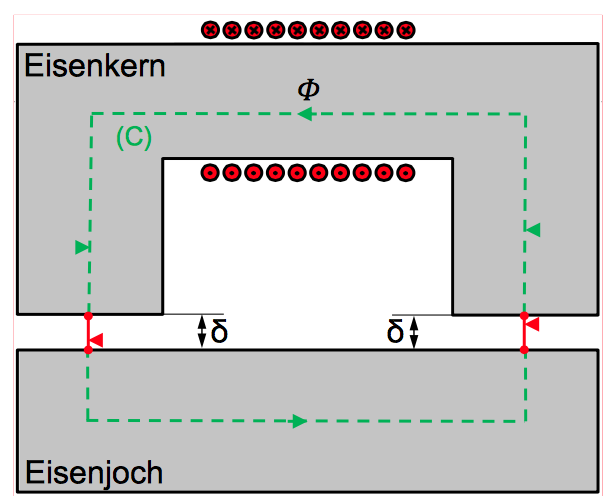
\includegraphics[width = \linewidth]{./Pics/VL2/magKreis}
\end{minipage}
\begin{minipage}{0.6 \linewidth}
Wenn der Magnetkern in der Stättigung ist, lässt sich das H-Feld im Eisen nicht mehr vernachlässigen: \\

$\oint_{(C)} \vec{H} \cdot \vec{dl} = H_{Fe} \cdot l_{Fe} + 2 \cdot \delta \cdot H_{\delta} $ \\

$H_{Fe} \cdot l_{Fe} + 2 \delta \cdot H_{\delta} = I \cdot N$ \\

$\Phi_{\delta} = \Phi_{Fe} \Rightarrow B_{\delta} = B_{Fe}$ \\

$H_{Fe} = \frac{B_{Fe}}{\mu_{Fe}} = \frac{B_{\delta}}{\mu_{Fe}} = \frac{\mu_0}{\mu_{Fe}} \cdot H_{\delta}$\\

$\frac{\mu_0}{\mu_{Fe}} \cdot H_{\delta} \cdot l_{Fe} + 2 \cdot \delta \cdot H_{\delta} = I \cdot N$\\

\textbf{$H_{\delta} = \frac{I \cdot N}{\frac{\mu_0}{\mu_{Fe}}+ 2 \delta}$}
\end{minipage}

\subsection{Permanentmagnet}

\begin{minipage}{0.3 \linewidth}
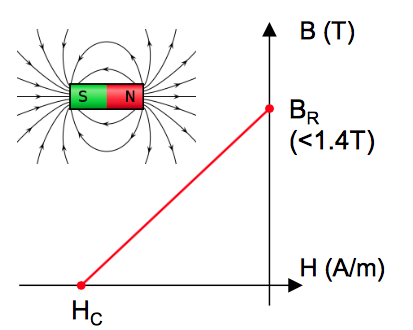
\includegraphics[width = \linewidth]{./Pics/VL2/permanentMagnet}
\end{minipage}
\begin{minipage}{0.7 \linewidth}
Ein Permanentmagnet (Dauermagnet) ist ein Stück eines magnetisierbaren Materials (Eisen, Kobalt, Nickel, Ferrit) welches sein statisches Magnetfeld behält ohne einen elektrischen Stromfluss. \\

Kennwerte der Dauermagnete:
\begin{itemize}
\item \textbf{Koerzitivfeldstärke $H_c$} Dieses Magnetfeld muss erzeugt werden um den Dauermagneten vollständig zu entmagnetisieren (B=0)
\item \textbf{Remanenz $B_R$} Das ist die magnetische Flussdichte des Dauermagnets ohne magnetisches Fremdfeld (H=0)
\item $B_m = \mu_m \cdot H_m + B_R , \mu_m = \mu_0$
\end{itemize}

Die Permanentmagneten ersetzen die Erregerspulen in den elektrischen Maschinen. Damit sind die Materialkosten und die ohmschen Verluste der Erregerspulen eliminiert. 
\end{minipage}

\subsubsection{Magnetkreis mit einem Dauermagneten (Allg. Herleitung)}
\begin{minipage}{0.4 \linewidth}
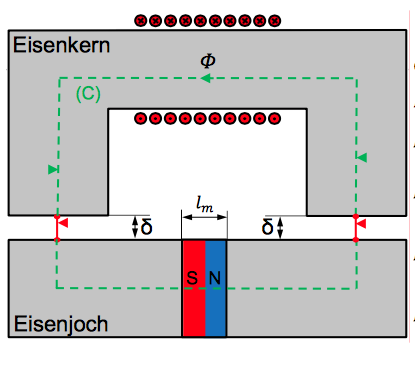
\includegraphics[width = \linewidth]{./Pics/VL2/permMagnet}
\end{minipage}
\begin{minipage}{0.6 \linewidth}
$\oint_{(C)} \vec{H} \cdot \vec{dl} = H_{Fe} \cdot l_{Fe} + H_{m} \cdot l_{m} + 2 \cdot \delta \cdot H_{\delta} $ \\

$H_{Fe} \cdot l_{Fe} + H_{m} \cdot l_{m} + 2 \cdot \delta \cdot H_{\delta} = I \cdot N$ \\

$B_m = B_\delta = B_{Fe}$ \\

$B_m = \mu_m \cdot H_m + B_R \Rightarrow H_m = \frac{B_m - B_R}{\mu_m}$ \\

$H_m =  \frac{\mu_0 \cdot H_\delta  - B_R}{\mu_m}$\\

$H_{Fe} = \frac{B_{Fe}}{\mu_{Fe}} = \frac{\mu_0}{\mu_{Fe}} \cdot H_\delta$\\

$H_m = \frac{\mu_0 \cdot H_\delta - B_R}{\mu_m}$\\

$H_{Fe} = \frac{B_{Fe}}{\mu_{Fe}} = \frac{\mu_0}{\mu_{Fe}}\cdot H_\delta $ \\

$\frac{\mu_0}{\mu_{Fe}} \cdot H_\delta \cdot l_{Fe} + \frac{\mu_0 \cdot H_\delta - B_R}{\mu_m} \cdot l_m + 2 \cdot \delta \cdot H_\delta = I \cdot N$

$H_\delta = \frac{I \cdot N + \frac{B_R}{\mu_m} \cdot l_m}{\frac{\mu_0}{\mu_{Fe}} \cdot l_{Fe} + \frac{\mu_0}{\mu_m} \cdot l_m + 2 \cdot \delta}$
\end{minipage}


\subsection{Reluktanzkraft}
\begin{minipage}{0.4 \linewidth}
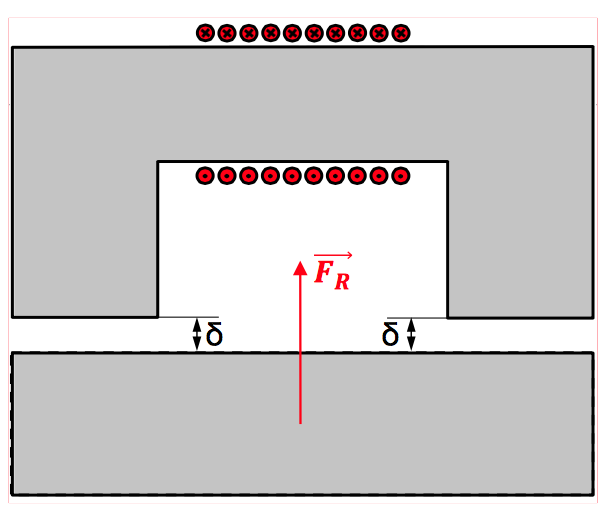
\includegraphics[width = \linewidth]{./Pics/VL2/reluktanz}
\end{minipage}
\begin{minipage}{0.6 \linewidth}
Die ferromagnetischen Körper sind im magnetischen Fremdfeld der so genannten Reluktanzkraft ausgesetzt. \\

Die Reluktanzkraft wirkt auf die ferromagnetischen Körper nur anziehen. \\

In dieser Anordnung lässt sich die Reluktanzkraft so angeben: \\

$F_R  = \mu_0 \frac{N^2 \cdot I^2 \cdot A}{4 \delta^2}$ \\

wobei A die magnetisch wirksame Fläche des Luftspalts ist. \\

Die magnetische Energie:\\

$W_m = \frac{1}{2} \cdot H_\delta \cdot B_\delta \cdot 2 \cdot A_{Fe} \cdot \delta= \mu_0 \cdot \frac{I^2 \cdot N^2}{4 \cdot \delta} \cdot A_{Fe}$ \\ 

wobei $A_{Fe} \cdot \delta$ das Volumen des Luftspalts ist. \\

Die Reluktanzkraft nach der Methode der virtuellen Verrückung: \\

$F_R = - \frac{\eth W_m}{\eth \delta} = \mu_0 \frac{I^2 \cdot N^2}{4 \cdot \delta^2} \cdot A_{Fe}$
\end{minipage}

\subsection{Zusammenfassung}

\begin{itemize}
\item Das magnetische Durchflutungsgesetz wird häufig für die Magnetfeldberechnung der stromdurchflossenen Spulen mit und ohne Magnetkreis eingesetzt. 
\item Ein Magnetkreis mit einer stromdurchflossenen Spule erzeugt einen magnetischen Fluss, der den entsprechenden Magnetfluss ohne Magnetkreis mehrere Grössenordnungen überschiesst.
\item Die magnetische Stromkraft wirkt auf einen stromführenden Leiter in einem fremden Magnetfeld.
\item Die magnetische Reluktanzkraft wirkt auf einen ferromagnetischen Körper im fremden Magnetfeld.
\item Die Permanentmagneten ersetzten stromdurchflossene Erregerspulen in den elektrischen Maschinen. Damit werden die Materialkosten und die ohmschen Verluste der Errgerspule eliminiert.
\end{itemize}




\end{document}
